%----------------------------------------------------------------------------------------
%	PACKAGES AND OTHER DOCUMENT CONFIGURATIONS
% %----------------------------------------------------------------------------------------

% singlespacing

\documentclass[11pt, english, openany, singlespacing, headsepline]{classes/ResearchTopic}

\usepackage[utf8]{inputenc} % Required for inputting international characters
\usepackage[T1]{fontenc} % Output font encoding for international characters
\usepackage{mathpazo} % Use the Palatino font by default
\usepackage{todonotes}
\usepackage{caption}
\newcommand{\hajj}[2][]{\todo[inline, color=green, author=elhajj, #1]{#2}}
% \usepackage[backend=bibtex,style=authoryear,natbib=true]{biblatex} % Use the bibtex backend with the authoryear citation style (which resembles APA)

\usepackage[%
    backend=biber,
    natbib=true,
    style=ieee, %apa of ieee?
    isbn=true,
    url=true,
    doi=true,
    % volume=true,
    % publisher=true,
    sorting=none
]{biblatex}

\addbibresource{references.bib} % The filename of the bibliography
\addbibresource{final-references-lit.bib} % The filename of the bibliography

\usepackage[autostyle=true]{csquotes} % Required to generate language-dependent quotes in the bibliography
\usepackage{nicematrix} % For Nicetabular table
\usepackage{calc}
% for multiple citation reference
% \usepackage{cite} 
% for managing images and figures
\usepackage{graphicx}
% For aligning table caption
\usepackage{caption}
% \captionsetup[table]{justification=raggedright,singlelinecheck=false}
% \captionsetup[table]{justification=raggedright,singlelinecheck=false, margin=0pt}
% \captionsetup[table]{position=above, format=hang, justification=raggedright, singlelinecheck=false}
% \captionsetup[table]{position=above, justification=justified, singlelinecheck=false}
\captionsetup[table]{singlelinecheck=false, justification=raggedright, margin=0pt, labelfont=bf}
\captionsetup[figure]{position=above, singlelinecheck=false, justification=raggedright, margin=0pt}

\newcolumntype{P}[1]{>{\raggedright\arraybackslash}p{#1\textwidth-2\tabcolsep-1.5\arrayrulewidth}}
\newcolumntype{Y}[1]{>{\centering\arraybackslash}p{#1\textwidth-2\tabcolsep-1.5\arrayrulewidth}}
\usepackage{tcolorbox} % for shadow box 
\usepackage{svg} % for svg 
\usepackage[export]{adjustbox} % to position image and table
\usepackage{parskip} % to disable automatic indentation and provide space between paragraphs 
% \usepackage{floatrow} % to put table label and caption above the table 
\usepackage{float}
\usepackage{threeparttable} % to put table label and caption above the table
\usepackage{svg} % To include svg figures
\usepackage{subcaption} % to put two images side by side
% \usepackage{graphicx}
\usepackage{adjustbox}
\usepackage{changepage}
\usepackage{smartdiagram}
\usepackage{longtable} % to make my table spans multiple pages 
\usepackage{changepage} % to change the offset of specific section of content 
\usepackage{booktabs}

\usepackage{pgfplots} %To add bar charts
\pgfplotsset{width=10cm,compat=1.9}

%---------------------------------------------------------------------------------------- 
% package and configuration for include c code.
\usepackage{xcolor}
\usepackage{listings}

\definecolor{mGreen}{rgb}{0,0.6,0}
\definecolor{mGray}{rgb}{0.5,0.5,0.5}
\definecolor{mPurple}{rgb}{0.58,0,0.82}
\definecolor{backgroundColour}{rgb}{0.95,0.95,0.92}

\lstdefinestyle{CStyle}{
    backgroundcolor=\color{backgroundColour},   
    commentstyle=\color{mGreen},
    keywordstyle=\color{magenta},
    numberstyle=\tiny\color{mGray},
    stringstyle=\color{mPurple},
    basicstyle=\footnotesize,
    breakatwhitespace=false,         
    breaklines=true,                 
    captionpos=b,                    
    keepspaces=true,                 
    % numbers=left,                    
    numbersep=5pt,                  
    showspaces=false,                
    showstringspaces=false,
    showtabs=false,                  
    tabsize=2,
    language=C
}

%---------------------------------------------------------------------------------------- 
--------------------------------------------------------------------------------------
% Configuration for drawing colorful table 
\usepackage{colortbl}

\newcommand{\mc}[2]{\multicolumn{#1}{c}{#2}}
\definecolor{Gray}{gray}{0.85}
\definecolor{LightCyan}{rgb}{0.88,1,1}

\newcolumntype{a}{>{\columncolor{Gray}}c}
\newcolumntype{b}{>{\columncolor{white}}c}

--------------------------------------------------------------------------------------
% 

%----------------------------------------------------------------------------------------
%	MARGIN SETTINGS
%----------------------------------------------------------------------------------------

\geometry{
	paper=a4paper, % Change to letterpaper for US letter
	inner=3.0cm, % Inner margin
	outer=3.8cm, % Outer margin
	bindingoffset=0.5cm, % Binding offset
	top=1.5cm, % Top margin
	bottom=1.5cm, % Bottom margin
	%showframe, % Uncomment to show how the type block is set on the page
}

%----------------------------------------------------------------------------------------
%	THESIS INFORMATION
%----------------------------------------------------------------------------------------

\thesistitle{Digital Twin and Securing IoT applications} % Your thesis title, this is used in the title and abstract, print it elsewhere with \ttitle
\supervisor{Dr.Ing Mohammed \textsc{El-hajj} T.M.  \textsc{ITÄPELTO}(Ph.D. Candidate )} % Your supervisor's name, this is used in the title page, print it elsewhere with \supname
\examiner{} % Your examiner's name, this is not currently used anywhere in the template, print it elsewhere with \examname
\degree{Master of Computer Science} % Your degree name, this is used in the title page and abstract, print it elsewhere with \degreename
\author{Teklit \textsc{Haphtu}} % Your name, this is used in the title page and abstract, print it elsewhere with \authorname
\addresses{} % Your address, this is not currently used anywhere in the template, print it elsewhere with \addressname

\subject{Cybersecurity, Computer Science} % Your subject area, this is not currently used anywhere in the template, print it elsewhere with \subjectname
\keywords{Digital Twin, Internet of Things, authentication} % Keywords for your thesis, this is not currently used anywhere in the template, print it elsewhere with \keywordnames
\university{\href{http://www.utwente.nl}{University of Twente}} % Your university's name and URL, this is used in the title page and abstract, print it elsewhere with \univname/
\department{\href{http://department.university.com}{Department of Computer Science}} % Your department's name and URL, this is used in the title page and abstract, print it elsewhere with \deptname
\group{\href{https://www.utwente.nl/en/eemcs/scs/}{SEMANTICS, CYBERSECURITY AND SERVICES (SCS)}} % Your research group's name and URL, this is used in the title page, print it elsewhere with \groupname
\faculty{\href{https://www.utwente.nl/en/eemcs/}{EEMCS}} % Your faculty's name and URL, this is used in the title page and abstract, print it elsewhere with \facname

\AtBeginDocument{
\hypersetup{pdftitle=\ttitle} % Set the PDF's title to your title
\hypersetup{pdfauthor=\authorname} % Set the PDF's author to your name
\hypersetup{pdfkeywords=\keywordnames} % Set the PDF's keywords to your keywords
}


\begin{document}

\frontmatter % Use roman page numbering style (i, ii, iii, iv...) for the pre-content pages

\pagestyle{plain} % Default to the plain heading style until the thesis style is called for the body content

%----------------------------------------------------------------------------------------
%	TITLE PAGE
%----------------------------------------------------------------------------------------

\begin{titlepage}
\begin{center}

\vspace*{.06\textheight}
{\scshape\LARGE \univname\par}\vspace{1.5cm} % University name
\textsc{\Large Master of Computer Science}\\[0.5cm] % Thesis type

\HRule \\[0.4cm] % Horizontal line
{\huge \bfseries \ttitle\par}\vspace{0.4cm} % Thesis title
\HRule \\[1.5cm] % Horizontal line
 
\begin{minipage}[t]{0.4\textwidth}
\begin{flushleft} \large
\emph{Author:}\\
\href{http://www.makeitsimple.com}{\authorname} % Author name - remove the \href bracket to remove the link
\end{flushleft}
\end{minipage}
\begin{minipage}[t]{0.4\textwidth}
\begin{flushright} \large
\emph{Supervisor:} \\
\href{https://people.utwente.nl/m.elhajj}{\supname} % Supervisor name - remove the \href bracket to remove the link  
\end{flushright}
\end{minipage}\\[3cm]
 
\vfill

\large \textit{A thesis submitted in fulfilment of the requirements\\ for the degree of \degreename}\\[0.3cm] % University requirement text
\textit{in the}\\[0.4cm]
\groupname\\\deptname\\[2cm] % Research group name and department name

\vfill

{\large \today}\\[4cm] % Date
%\includegraphics{Logo} % University/department logo - uncomment to place it
 
\vfill
\end{center}
\end{titlepage}

%----------------------------------------------------------------------------------------
%	LIST OF CONTENTS/FIGURES/TABLES PAGES
%----------------------------------------------------------------------------------------

\tableofcontents % Prints the main table of contents

\listoffigures % Prints the list of figures

\listoftables % Prints the list of tables

%----------------------------------------------------------------------------------------
%	THESIS CONTENT - CHAPTERS
%----------------------------------------------------------------------------------------

\mainmatter % Begin numeric (1,2,3...) page numbering

\pagestyle{thesis} % Return the page headers back to the "thesis" style

% Include the chapters of the thesis as separate files from the Chapters folder

% Chapter 1

\chapter{Introduction} % Main chapter title

\label{Chapter1} % For referencing the chapter elsewhere, use \ref{Chapter1} 

%----------------------------------------------------------------------------------------
% Define some commands to keep the formatting separated from the content 
\newcommand{\keyword}[1]{\textbf{#1}}
\newcommand{\tabhead}[1]{\textbf{#1}}
\newcommand{\code}[1]{\texttt{#1}}
\newcommand{\file}[1]{\texttt{\bfseries#1}}
\newcommand{\option}[1]{\texttt{\itshape#1}}

%----------------------------------------------------------------------------------------
% 
% \hajj{Chapter One introduces the topic of the thesis to the reader. The critical part of writing Chapter One is to establish the statement of the problem and research questions. Basically, you are justifying to the reader why it is nec- essary to study this topic and what research question(s) your study will answer. Usually, the topic is based around a particular problem area that you want to focus on. However, before you introduce the reader to the specific topic and problem, you have to first provide the reader with the broader context (the general problem) and consequences related to the topic. In other words, before you discuss the specific problem, you need to contextualize your topic within the larger problem. For example, you would first discuss the problems related to the topic.
% Chapter One of the thesis includes a section on the Statement of the Problem (information about the specific problem), Background and Need (the background literature related to the problem), the Purpose of the Study (the focus and goal of the study), Research Questions (what questions the study proposes to answer), and other significant sections. In this chapter, you need to support all of your claims and positions using citations
%  check this reference please:
%  https://www.wcupa.edu/business-publicManagement/geographyPlanning/documents/thesisGuideline.pdf}
% \begin{enumerate}
    %item state the general topic and give some background
    %\item provide a review of the literature related to the topic
        % \item define the terms and scope of the topic
        % \item outline the current situation
        % evaluate the current situation (advantages/ disadvantages) and identify the gap
    % \item identify the importance of the proposed research
    % \item state the research problem/ questions
    % \item state the research aims and/or research objectives
    % \item state the hypotheses. DONE
    % \item outline the order of information in the thesis. DONE
    % \item outline the methodology. DONE
% \end{enumerate}


% General Research topic 
\section{Research Topic}We are in an era where it is difficult for industries and organizations to run a business process without connectivity and data exchange. With the advent of Industry 4.0, Digital Twins(DT) and Internet of Things(IoT) are the two enabling technologies that provide unprecedented levels of connectivity and data exchange to monitor and optimize business operation. Both technologies have been around for a while, but the integration of of them is just getting started.

\section{Literature Review}
% Methodology Summary 
% The core concept of Digital Twin
% How digital twin is used to securing IoT application 
% How data is secure 
This study conducted a systematic literature review to investigate the use of Digital Twin in enhancing the security of IoT applications in industry 4.0. The review followed a three-phase approach, including using automated tools for the review process. A total of 523 papers were initially collected from seven digital libraries, and after applying inclusion and exclusion criteria and quality assessment, 57 relevant papers were selected for the review. 

The definition of digital twins in the literature varies depending on the context, but generally, it consists of three components: physical and digital states, interconnectivity, and a process for collecting and examining data.

The use cases for digital twins are vast, including threat detection and response, vulnerability assessment, security awareness training, and threat intelligence. A wide range of industry 4.0 sectors benefit from this technology, including the power grid, automotive industry, water treatment plants, transportation systems, and satellite internet, among others. Researchers have deployed security-enabled digital twins to improve the security and safety of operations.  
Machine learning and data analytics are the two primary technologies widely used by study authors to enable digital twin security features. Other technologies, such as blockchain, cloud computing, and federated learning, are also used. However, most authors neglect the security concerns related to the data used by digital twins during transmission and while at rest.  
Some researchers have proposed encryption methods, such as AES and RSA, to secure digital twin data. However, these methods may not be feasible for deployment in device-constrained devices. Other researchers have suggested using blockchain to maintain the integrity and reliability of data shared by a network of digital twins.  

% Niche
\section{Niche and Scope}
Internet of Things (IoT) is a network of physical objects, such as smart devices, sensors, actuators, vehicles, and buildings powered by software and network connectivity that allows them to collect and exchange data[\textcolor{red}{ref}]. Digital Twin can be described as software defined digital representation of physical object that receive large set of sensor data about environment and operating condition to simulate and monitor operation in real-time\cite{williamdanilczykANGELIntelligentDigital2019, danilczykSmartGridAnomaly2021}. Simulation of an operation, visualization of product in real-time, troubleshooting remote equipment, and managing assets in industry are a few of the use cases among the others. Together, those two technologies are transforming the way we manage resources and operations. 

% The importance of this research
% The challenge in story telling scenario 
\section{Importance of the Research}
Digital Twin and IoT have an important role to play in various sectors including industries, critical infrastructures, health, smart cities, and so on. Therefore, during the interaction or communication, it is important to ensure the security of those two technologies. Authentication is a critical security principle that can come to rescue to address the aforementioned concern by only allowing an authorized end point to access system and data. In other words, in context of Digital Twin and IoT, authentication can enable us to make sure only known IoT device can send sensor data to Digital Twin hub and only known Digital Twin send command to device situated remotely. Without authentication, a malicious user can gain access to a system, leading to serious security problems. 

\
% Problem statement 
\section{Problem Statement}
As noted previously, manufacturing facilities, including critical infrastructure, are using an IoT device to collect and send sensor measurement and operating conditions to the Digital Twin station to monitor and optimize the overall operation of the business process. However, due to the storage and processing constraints that IoT devices have [ \cite{williams_survey_2022}, \cite{noauthor_lightweight_nodate}], it is challenging to adopt traditional security cryptographic mechanisms to ensure the confidentiality and integrity of the data flow between IoT and DT. If proper security measures (authentication, authorization, encryption, and so on) are not used, an attacker may be able to perform a man-in-the-middle attack with the intent of intercepting sensitive sensor data or disrupting a system by injecting his crafted faulty data\cite{salimBlockchainEnabledSecureDigital2022}. In recent literatures and blog of standard institutes, it is mentioned to utilize security schemes that can fit into constraint devices to address the security requirement.  

% Proposed Solution and Hypothesis 
\section{Proposed Solution}
In this study, we propose a lightweight mutual authentication scheme , based on NIST standardized authentication encryption, to ensure the security requirement of IoT applications and Digital Twin. Our authentication scheme will enhance the confidentiality and integration of the communication channel between the Digital Twin and its counter physical component. In addition, we envision that our mutual lightweight authentication scheme can also provide secure access to remote IoT device(sensors) and  Digital Twin station. 

\section{Research Objective and Aims}
This research has two main objectives. First, through systematic literature review, analyze the core concept of a Digital Twin and synthesis the information presented in the literature on how DT is used to enhance the security of IIoT/IoT application in industry 4.0 use cases. Second, with the objective of implementing NIST standard light-weight authentication scheme, we aim to improve the security of a digital communication that is established between power, storage, and processing constraint devices and DT statation hosted on cloud or local premises. In the context of industry 4.0 uses cases,  IIoT devices are field devices such as sensors and actuators situated in a remote industry zone where it is not convenient to reach and access them. Hence, it is important to implement an efficient and performant cryptographic solution to increase the life-longevity of these power constraints devices to avoid periodic repairs or replacement.  

\section{Hypothesis}
% More security
% efficiency increase speed of data flow 
% Getting a real time of data is one requirement of DT application 
Getting real-time and authentic data from sensors is one requirement of DT application \cite{yuchenziqianzhangningtangApplicationDigitalTwin2022}.In this sense, implementing a lightweight authentication scheme will enhance security and increase the speed of data flow between DT and IIoT sensors. In addition, our scheme can provide remote secure access to IoT and DT.  


% Methodology 
\section{Methodology}
This study has two major part;literature review and implementation of proposed solution. For the literature review, we conducted a systematic way of reviewing previous leiteratures with the aim of synthesizing the core concept of Digital Twin and analyzing the existing solution for securing IoT application using Digital Twin. To implement our proposed solution, which is a lightweight authentication scheme, we leverage platform called Ditto and microcontroller manufactured by Pycom called ESP32. Ditto is an open source framework developed and maintained by Eclipse Foundation to facilitate the interaction between Digital Twin and IoT devices\cite{noauthor_eclipse_nodate}.ESP32 microcontroller is a chipset that can be programmed with micropython which is an implementation of Python3 for microcontroller. 
The performance and efficiency of our proposed solution is validated, at the end of the study, by measuring the power consumption, execution time, and storage complexity. 

\begin{figure}[H]
    \centering
    \includesvg[width=\textwidth]{images/svg/ps-scheme-final.svg}
    \caption{Proposed solution schemes and experiment context}
    \label{fig:ps-scheme}
\end{figure}

% outline the order of information in the thesis 
\section{Report outline}
The remainder of this study report is organized as follow. In the following section, we present the methodology we imploy for the systematic literature review process. Then we provide details of the results of the literature review. Following that, we discuss the summary of the result and limitations of the study. Finally, we draw our conclusion on the basis of the evidence we gathered.   

% The emergence of Digital Twins(DT) and the Internet of Things(IoT) has opened up a new opportunity for businesses to take advantage of technology to gain insights and optimize performance. To maintain the security and privacy of data, these technologies come, however, with their own unique set of security challenges that must be addressed. In this paper, we will explore the current state of security, particularly the authentication scheme used to ensure the confidentiality and integrity of data flow between the virtual model;the digital twin, and the physical devices, which could be sensors or actuators. We will also provide lightweight DT based authentication scheme along with how to implement for IoT application. Finally, we will conclude our work with a recommendation on how to protect a DT and IoT network with efficient and performant cryptographic authentication schemes.


% Chapter 2
\chapter{Literature Review Methodology} % Main chapter title

\label{Chapter2} % For referencing the chapter elsewhere, use \ref{Chapter1} 

Based on the guidance obtained from a previous investigation on how to conduct a literature review, the authors decided to perform a systematic analysis of the existing literature. In this process, specific protocols and techniques are clearly described so that other researchers can replicate the study and get the same results. 

After conducting preliminary research on how to conduct a literature review, we made the decision to perform a systematic analysis of existing literature in order to answer two out of the four research questions. Systematic Literature Review(SLR) is a formal and structured process of synthesize existing research studies that are relevant to answer pre-defined research questions \cite{kitchenham_guidelines_2007}. Its purpose is to provide a comprehensive overview of the current state of the literature and identify research gaps \cite{carrera-rivera_how-conduct_2022}. Conducting an SLR allows researchers to gain valuable insights into a particular field or topic, and to build upon existing research by identifying areas that require further investigation.

Furthermore, we adhered to the three-phase approach of conducting a systematic literature review as outlined by Kitchenham and Charter \cite{kitchenham_guidelines_2007}, which includes planning protocol, conducting review, and reporting results. This approach ensures that the systematic literature review is conducted in a structured and transparent manner according to Kitchenham and Charter \cite{kitchenham_guidelines_2007}. Using this guideline and additional resources, we present a flow diagram of our reviewing process is depicted in Figure \ref{fig:slr-proc}. 

In this study, the literature review has two main objectives. The first objective is to identify existing solutions that leverage DT to enhance the security of (I)IoT applications. The second objective is to identify the security mechanisms employed to secure the data which could be at rest or in transmission between the digital twin station and the data source ((I)IoT devices)



\begin{figure}[H]
    \centering
    \caption{A flow diagram of the review process.}
    \includegraphics[width=0.9\textwidth]{images/slrmethoddiagram.drawio.png}
    % \includesvg[width=1\textwidth]{images/svg/slrmethoddiagram.drawio.svg}
    
    \label{fig:slr-proc}
\end{figure}


To automate the systematic literature review process, from defining PICOC to data extraction, we use a web tool called\textit{parsif.al}\footnote{\href{https://parsif.al}{Parsifal} is an online tool designed to support researchers in performing systematic literature reviews in the context of software engineering. Geographically distributed researchers can work together within a shared workspace, designing the protocol and conducting the research}


\section{Review Protocol}
According to Kitchenham and Charter  \cite{kitchenham_guidelines_2007}, it is essential to define a review protocol that outlines the procedures and methods before beginning the review process. The protocol serves as a road-map for conducting the review and ensures that the study can be replicated by providing a clear and detailed plan of the procedures to be followed \cite{carrera-rivera_how-conduct_2022}.

% \subsection{PICOC and Synonyms}
%----------------------------------------------------------------------------------------
% ======================================================================================================
% NOTES, TODOS
% ======================================================================================================

\subsection{Defining PICOC}
PICOC stands for Population, Intervention, Comparison, Output and context. It is a widely used technique in medical and social science studies to define the focus of the research\cite{carrera-rivera_how-conduct_2022}. However, in\cite{carrera-rivera_how-conduct_2022, kitchenham_guidelines_2007} Kitchenham and Carrera showed that this technique can still be applied for computer science related research to formulate and structure research questions. In this subsection, we define our PICOC criteria for this systematic literature review.

\textit{Population:} The motivation to conduct this research is the security related problem we identified in the communication between Digital Twin and constrained  (I)IoT devices deployed in the smart industry to collect sensor data. Hence, the problem domain or "Population" for this research is (I)IoT devices used with Digital Twin to enhance security in Industry 4.0. Industries that use Digital Twin and (I)IoT devices, such as smart cities, smart homes, smart grids, smart health, smart manufacturing, etc. In this sense, the "Population" part of PICOC in this review refers to the following terms: Digital Twin, (Industrial)Internet of Things, Industry 4.0, Smart Manufacturing, Cyber-physical Systems, and Critical Infrastructure. 

\textit{Intervention:} Our intervention to address this problem, the security issue of digital communication between Digital Twin and (I)IoT, is to implement a lightweight NIST standard cryptographic authentication/encryption scheme for power and computation constraint (I)IoT devices. In this regard, we use the term "authentication" as an intervention.

\textit{Comparison:} Before designing and implementing an intervention for a specific problem, it is important to identify the existing solution in the literature. The results of reviewing, comparing and analysing the existing solution discussed in the relevant research literature can be used as input to design and implement the intervention methodology. With this regard, this study will identify and compare authentication schemes or security mechanisms used in securing a data flow between Digital Twin and (I)IoT. 

\textit{Outcome:} Secure remote access with integrity and confidentiality of communication, efficient and performant cryptographic schemes that can run on constrained devices is the expected outcome of this research.\\

\textit{Context:} This systematic literature review is focused on the Industry 4.0 environment, targeting Digital Twin solutions deployed in smart industries to enhance security. However, the second part of the study is dedicated to designing and implementing authentication schemes for the Smart Grid which is considered as one instance of Industry 4.0.
%----------------------------------------------------------------------------------------


% \subsection{Research Questions}
%----------------------------------------------------------------------------------------
% ======================================================================================================
% NOTES, TODOS
% ======================================================================================================

\subsection{Research Question}
Before embarking on the process of identifying studies and extracting data, it is crucial to identify and clearly define research questions or objectives, as they serve as guiding principles for conducting a literature review\cite{carrera-rivera_how-conduct_2022}. Consequently, this systematic literature review aims to address the following research questions:

\begin{itemize}

    % RQ1
    \item \textbf{RQ1: How is Digital Twin used to enhance the security of (I)Iot applications in the industry 4.0 use cases ?} - 
    this question aims to identify how Digital Twin is used to improve the security of industries that use IoT devices, including sensors and actuators, to achieve OT (operational technology) security goals: Safety, reliability, and availability.
    % \begin{itemize}
    %     % I need a comment from Mohammed on this -> with regad to use case -> is to braod and vogue?
    %     \item \textbf{RQ1.1: What is the concrete concept of Digital Twin} - 
    %     under subcategory of the above research question, the concept of digital and its use cases are explored.
    % \end{itemize}

    % RQ 1
    % \item RQ1. What mututal authentication schemes for DT and IoT application are discussed in the literature? 
    % \item How can we use Digital Twin to enhance security issue in IoT/IIoT application? 
    %  Replace schemes by  mechansims.
    \item \textbf{RQ2: What are the security methods presented in the literature to ensure the authentication between Digital Twin and its mapped physical devices?} - 
    this question focus on the identification of authentication mechanisms that are used to ensure the security of DT and (I)IoT communication.
\end{itemize}
%----------------------------------------------------------------------------------------

% \subsection{Key Terms and Search Strategy}
%----------------------------------------------------------------------------------------
% ======================================================================================================
% NOTES, TODOS
% ======================================================================================================
% Define the search strategy for each database if possible 
% Also prepare table with or and operators refer poatek
% I need to modify the title and the resarch question -> Iot to IIoT , the area is in manufcturing or Industry 4.0.
% receive comment on the keyword variants. example IIoT, schemes.
% =======================================================================================================
\subsection{Search keys and Strategies}
Guided by the PICOC criteria and  research questions, we construct four main search strings to create search queries used for each selected databases. These are, "Digital Twin" "IoT" "Authentication", and "Industry". Synonyms, alternative spellings, and similar semantic meanings are considered for each keyword and combined using OR operator. 

During pilot search, on majority of databases, we identified adding synonyms of "Digital Twin" does not return new paper compared to searching using only the term "Digital Twin". Hence, we avoided to use other "Digital Twin" synonym terms for simplicy of our search query. 

\begin{table}[h]
% \captionsetup{
%   justification=raggedright,
%   singlelinecheck=false,
%   margin=60pt % adjust margin as needed
% }
% \centering
\caption{ Key terms and key variants.}
\begin{NiceTabular}{p{3.2cm}p{11cm}}
\toprule
    \textbf{Key terms} & \textbf{Variants / Synonyms / Similar Semantic Meaning} \\
    \midrule
    Digital Twin & DT, digital-twin, digital-twins, digital replica, digital shadow, virtual model, virtual clone \\ \hline
    (Industrial)Internet of Things & IoT, IIoT, internet-of-things, internet-of-thing, industrial internet of things, industrial-internet-of-thing, sensors, actuators, smart devices  \\ \hline
    Authentication & security, confidentiality, certificate, verification, scheme, schemes\\ \hline
    Industry & industry 4.0, manufacturing, smart manufacturing, factory, smart factory, cyber-physical system, cyber-physical systems, cyber physical systems, cyber physical system, critical infrastructure, critical infrastructures. \\ 
\bottomrule
\end{NiceTabular}
\end{table}

% As an example, an advance search query for Scopus databases is shown in table \ref{}.\\


% \begin{table}[h]
% % \centering
% \caption{\label{scopus-advanc-search} Example of advanced search query in Scopus}
% \begin{NiceTabular}{Y{1.1}}
% \CodeBefore
%   \rowcolor{gray!50}{1}
%   \rowcolors{2}{gray!25}{white}
% \Body
%  ("dt" OR "digital twin" OR "digital twins" OR "digital-twin" OR "digital-twins" OR "digital replica" OR "digital shadow" OR "virtual model" "virtual clone")  \\
%  AND \\
%  ("internet of things" OR "internet of thing" OR "internet-of-thing" OR "internet-of-things" OR "IIoT" OR "industrial internet of things" OR "industrial-internet-of-thing" OR "sensors" OR "actuators" OR "smart devices" )  \\
%  AND \\
% ("security" OR "authentication" OR "certificate" OR "verification" OR "schemes") \\
%  AND \\
% ("industry" OR "industry 4.0" OR "manufacturing" OR "smart manufacturing" OR "factory" "smart factory" OR "cyber-physical systems" OR "cyber-physical system" OR "cyber physical system")  \\
% \end{NiceTabular}
% \end{table}
%----------------------------------------------------------------------------------------

% \subsection{Digital Library}
%----------------------------------------------------------------------------------------
% ======================================================================================================
% NOTES, TODOS
% ======================================================================================================
% One paragraph about the databases 
% A table that show description and reason for selection
\subsection{Digital Library Sources}

In an attempt to perform an exhaustive search on literature that has relevant studies to our research question, we leverage six electronic archives (databases) that are known in publishing papers on computer science. These are ScienceDirect, SpringerLink, Scopus, IEEExplore, ACM, and WebofScience.  Six of them were selected in accordance with quidelines provided by Kofod \cite{kofod-petersen_how_nodate} and Kitchenham \cite{kitchenham_guidelines_2007}. 




%----------------------------------------------------------------------------------------

% \subsection{Inclusion and Exclusion Critera}
%----------------------------------------------------------------------------------------
% ======================================================================================================
% NOTES, TODOS
% ======================================================================================================

\subsection{Inclusion and Exclusion Criteria }
\label{sec:inc-exc}


\textit{Inclusion}: We only considered studies written in English, easily accessible in full text, and published in journals or conferences in the field of computer science between 2016 and 2022. 

\textit{Exclusion:} Any studies that did not meet the inclusion criteria, including those written in a language other than English, not accessible in full text, classified as gray literature, published before 2016, or not related to computer science or our research questions, were excluded from the selection process. The inclusion and exclusion criteria utilized for the purpose of filtering research studies from the search results of databases are presented in Table \ref{tbl:table-inc-exc}. 


\begin{table}[H]
\centering
\caption{\label{tbl:table-inc-exc}Inclusion and exclusion criteria.}
\begin{NiceTabular}{p{3cm}p{6cm}p{5cm}}
\toprule
    \textbf{Criteria Type} & \textbf{Inclusion} & \textbf{Exclusion} \\
    \midrule
    \textbf{Period} & Studies published between 2016 and 2022 & before 2016 \\ 
    \textbf{Language} & English & Not English \\
    \textbf{Accessibility} & accessible in full-text & Not accessible in full-text \\ 
    \textbf{Type of source} & Journal articles, conference proceedings  & Books, book chapter, \\ 
    \textbf{Type of literature} & Of type black literature & Grey literature  \\ 
    \textbf{Relevance} & Study related to computer science & Not related to computer science \\
\bottomrule
\end{NiceTabular}
\end{table}


%----------------------------------------------------------------------------------------

%----------------------------------------------------------------------------------------
% ======================================================================================================
% NOTES, TODOS
% ======================================================================================================
% describe how to perform the detail assessment
% use numeral scale 
% Are the aim of the article clearly stated?
% Is the implementation detail explained adequately 
% does the study has direct link to research question 1 and/or question 2. 
% 
\subsection{Quality Assessment Checklist}
Beside the inclusion and exclusion criteria, it is important to evaluate the quality of the research study [kitchen]. Quality assessment checklist define the detail assessment criteria for selecting paper during screening abstract and introduction of the paper. In this stage, articles that are not relevant to the research question and the objective of the study are identified and removed [kofod]. 

Below, we outline quality assessment questions as a checklist. 
\begin{itemize}
    \item \textbf{QA1:} Does the study clearly define the aim and objective of the research?
    \item \textbf{QA2:} Does the study fully explain a methodology to secure IoT/IIoT application using Digital Twin
    \item \textbf{QA3:} Does the study has direct link to research question 1 and / or question 2?
    \item \textbf{QA4:} Does the study conducted an experiment(test) to validate the hypothesis? 
    \item \textbf{QA5:} Does the study provide detail implementation of authentication scheme?
    
\end{itemize}
The quality assessment questions outlined above were evaluated using a numerical metric scoring system, with a range of 1-5, where 1 represents an irrelevant article and 5 represents a highly relevant and qualified article. The level of agreement in answering the quality checklist questions was determined through a categorical classification system, comprising of "Agree," "Somewhat Agree," "Neutral," "Somewhat Disagree," and "Disagree." These categories were assigned corresponding weight values, with "Agree" being assigned the highest weight value of 5 and "Disagree" being assigned the lowest weight value of 1. This scoring system helped to make sure that we were evaluating the research studies in a fair and consistent way, so that the studies that were most relevant and of the highest quality were selected for the review.

%----------------------------------------------------------------------------------------

% \subsection{Defining Data Extraction Form}
%----------------------------------------------------------------------------------------
% ======================================================================================================
% NOTES, TODOS
% ======================================================================================================

\subsection{Data Extraction Form}
According to Kitchenham et al.\cite{kitchenham_guidelines_2007}, a well design data extraction form is crucial for collecting information from selected primary studies to address research questions. In this study we use parsif.al web tool to design and structure data extraction form for collecting data from selected papers.  

The data extraction form is continuously evolving during the full-text review process. 

More data to be filled..... A table with data extraction from will be drawn here. 
%----------------------------------------------------------------------------------------


\section{Conducting Review}

In this study, a total of 523 articles were retrieved from online digital databases, namely ScienceDirect, SpringerLink, Scopus, IEEExplore, ACM, and Web of Science, which are known for publishing computer science-related research studies.

For all databases, we limit the search result based on inclusion/exclusion criteria defined in section \ref{sec:inc-exc}. To recall , we included only papers published between 2016 and 2023 in the field of computer science, and document-type articles from journals and conferences were considered for the final search result.

Furthermore, different search queries and strategies were used for each selected database, as they have different search mechanisms. 

% \subsection{Search Queries and Search Strategy}
%----------------------------------------------------------------------------------------
% ======================================================================================================
% NOTES, TODOS
% ======================================================================================================
\subsection{Search Queries and Search Strategy}

 Each of the selected database comes with their own way of performing advance searching. The search field and filtering option are different from one database to another. Having this into consideration, we design a search strategy we called bottom down three stage searching mechanism. The detail at each stage is explained as follow. 

First we look for the main key term -- Digital twin -- on the title of the paper. The assumption behind this is that if the research main focus is digital twin it is highly likely that its title contains digital twin. Since our main objective is to understand how digital twin is used to secure IoT application on various sectors, we then narrow the previous search result by looking for security related terms such as "authentication", "security", "encryption", and "cryptography" on the abstract. In the third stage, if the number of retrieved papers is greater than 30, we further narrow the search result by tuning our search query to look for IoT and industry related terms in the full text of the research paper. 

\begin{tcolorbox}[colback=black!5!white, sharp corners=all, colframe=white!95!black]
\textbf{Web of Science}
\tcblower
("digital twin*" OR "digital-twin*") (Title) AND ( "authenticat*" OR "cryptography" OR "security" OR "encrypt*" ) (Abstract) and English (Languages) and Article or Proceeding Paper (Document Types) and Engineering or Computer Science (Research Areas)
\end{tcolorbox}

In Web of Science, "Topic"(i.e Title, keyword, and Abstract) filed is used to search for digital twin and internet of things terms. The security related terms like authentication, encryption, cryptography and encryption as well as terms related to industry are searched on all fields. From the search results of our query, document types such as book chapters, early access,and editorial are excluded. In other words, only document of type article and conference papers are selected. We run the search query over all available years which are published under category of computer science and 30 articles are returned as a result.
\begin{tcolorbox}[colback=black!5!white, sharp corners=all, colframe=white!95!black]
\textbf{Scopus}
\tcblower
( TITLE ( ( "digital twin*" OR "digital-twin*" ) ) AND TITLE-ABS-KEY ( "authenticat*" OR "cryptography" OR "security" OR "encrypt*" ) AND TITLE-ABS-KEY ( ( "industr*" OR "Industry 4.0" OR "factor*" OR "manufactur*" OR "smart manufacturing" OR "cyber-physical system*" OR "cyber physical System*" OR "infrastructure*" OR "industrial control system*" ) ) ) AND ( LIMIT-TO ( SUBJAREA , "COMP" ) OR LIMIT-TO ( SUBJAREA , "ENGI" ) ) AND ( LIMIT-TO ( DOCTYPE , "cp" ) OR LIMIT-TO ( DOCTYPE , "ar" ) ) AND ( LIMIT-TO ( SRCTYPE , "p" ) OR LIMIT-TO ( SRCTYPE , "j" ) ) AND ( LIMIT-TO ( LANGUAGE , "English" ) )
\end{tcolorbox}
We employ the same search methodology and search terms for Scopus as we do for Web of Science. We run our query string with intention to find terms in "Article title", "Abstract" and "Keywords". While document type article and conference paper are included; conference review and book chapter are excluded. Our search result returned 97 articles in total. 

\begin{tcolorbox}[colback=black!5!white, sharp corners=all, colframe=white!95!black]
\textbf{IEEExplore}
\tcblower
("Document Title":"digital twin*" OR "Document Title":"digital-twin*") AND ("Abstract":"authenticat*" OR "Abstract":"cryptography" OR "Abstract": "security" OR "Abstract":"encrypt*") \\

Filters Applied: Conferences Journals
\end{tcolorbox}
In the case IEEE, we use a different search strategy from the above two cases. while we perform search for terms  authentication and industry related on full text , the "All Metadata" field is used to perform the others search terms on title, keywords, and abstract. Articles from conferences and journals are selected and articles under category of early access and magazines are excluded. Finally, Our query resulted in 37 research studies.   

\begin{tcolorbox}[colback=black!5!white, sharp corners=all, colframe=white!95!black]
\textbf{ACM}
\tcblower
[[Title: "digital-twin*"] OR [Title: "digital twin*"]] AND [[Abstract: "security"] OR [Abstract: "authenticat*"] OR [Abstract: "encrypt*"] OR [Abstract: "cryptography"]]

\end{tcolorbox}
ACM is a bibliographic database that exclusively focuses on publishing computing literature. In ACM we run the search query within the search field of "Anywhere". And only research articles are included, and as a result 12 research studies are retrieved. 





%----------------------------------------------------------------------------------------


% \subsection{Search Result and Bibliometric Analysis}
%----------------------------------------------------------------------------------------
% ======================================================================================================
% NOTES, TODOS
% ======================================================================================================
\subsection{Search Result and Bibliometric Analysis}
Following the selection process using the inclusion and exclusion criteria, and the removal of duplicate studies, a total of 74 research papers were considered for further review and analysis. Of these, 44(60\%) were conference papers, while the remaining 40\% were journal articles.

The Majority of the selected papers were retrieved from Web of Science and Scopus, with approximately 41\% and 23\% respectively, as both are the major citation databases. Furthermore, a notable proportion of papers were also obtained from other sources, including the IEEE Digital Library (15.1\%), Springer Link (11\%), ACM Digital Library (6.8\%), and Science Direct (2.7\%). These finding are illustrated in Figure \ref{fig:archive-itemtype}, using pie chart in terms  of document type and source archive. These chart highlight the importance of leveraging a wide range of digital archives to ensure a comprehensive review of the literature. 

% \begin{figure}
% \includesvg[width=0.5\textwidth]{images/svg/databases.svg}
% \includesvg[width=0.5\textwidth]{images/svg/itemtype.svg}
% \svgcaption{This is the label for the SVG image.}
% \label{fig:image}
% \end{figure}

\begin{figure}[H]
    \centering
    \begin{subfigure}[b]{0.45\textwidth}
        % \includegraphics[width=\textwidth]{image1.png}
        \includesvg[width=\textwidth]{images/svg/databases.svg}
        \caption{Percentage of papers per database}
    \end{subfigure}
        \begin{subfigure}[b]{0.45\textwidth}
        % \includegraphics[width=\textwidth]{image2.png}
        \includesvg[width=\textwidth]{images/svg/itemtype.svg}
        \caption{Proportion of papers per item type}
    \end{subfigure}
    \caption{Paper distribution}
    \label{fig:archive-itemtype}
\end{figure}


Analysis of the distribution of selected papers based on publication year revealed that the majority of articles were published in 2022 and 2021. Furthermore, the bar chart illustrates a general upward trend in the number of publications addressing security concerns for industries utilizing Digital Twin and (I)IoT applications. This trend indicates that there is a growing interest and concern among researchers in the field of Digital Twin and IoT security, and highlights the relevance and timeliness of this systematic literature review.

\begin{figure}[H]
    \includesvg[width=0.9\textwidth]{images/svg/pub_year_white_bg.svg}
    \caption{Number of published papers per year}
    \label{fig:bar-chart-yaer}
\end{figure}
% \hajj{please remove the background color of the figure}
To gain a deeper understanding of the trending topics within the 74 selected papers published between 2018 and 2023, a frequency analysis of keywords was conducted. This analysis was performed by extracting keywords that appeared more than three times in the abstracts and keyword sections of the articles, using the VOSviewer tool. Further filtering and sensitization was applied to create a shortlist of keywords. Additionally, keywords which have similar meanings with different spellings and variations were merged. The resulting frequency analysis of keywords, illustrated in Figure \ref{fig:alluvial-key}, provides valuable insights into the key themes and concepts that are prevalent in current research on the topic of Digital Twin and IoT security. This analysis can help guide future research by identifying areas where there is a need for further investigation and providing a sense of the current state of the field.


\begin{figure}[H]
    % \includesvg[width=0.9\textwidth]{images/svg/key_buble.svg}
    % 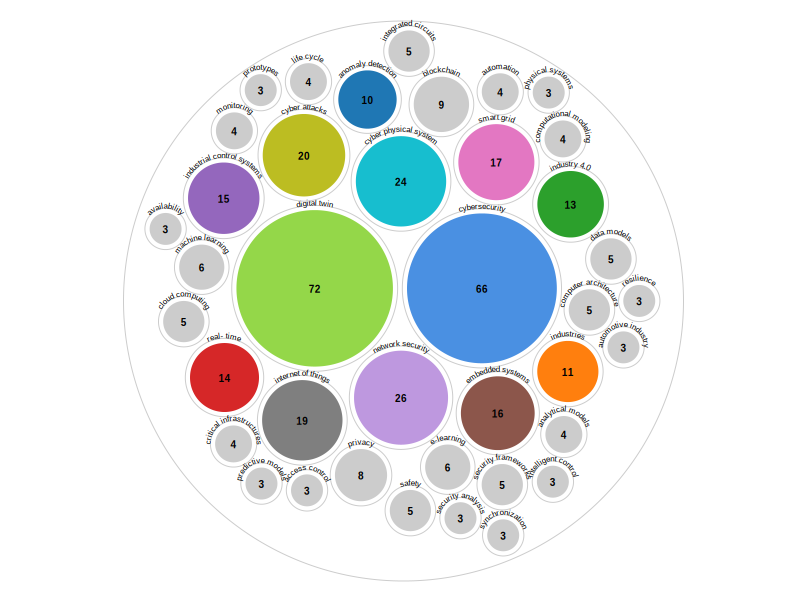
\includegraphics[width=\textwidth]{images/svg/key_buble.png}
    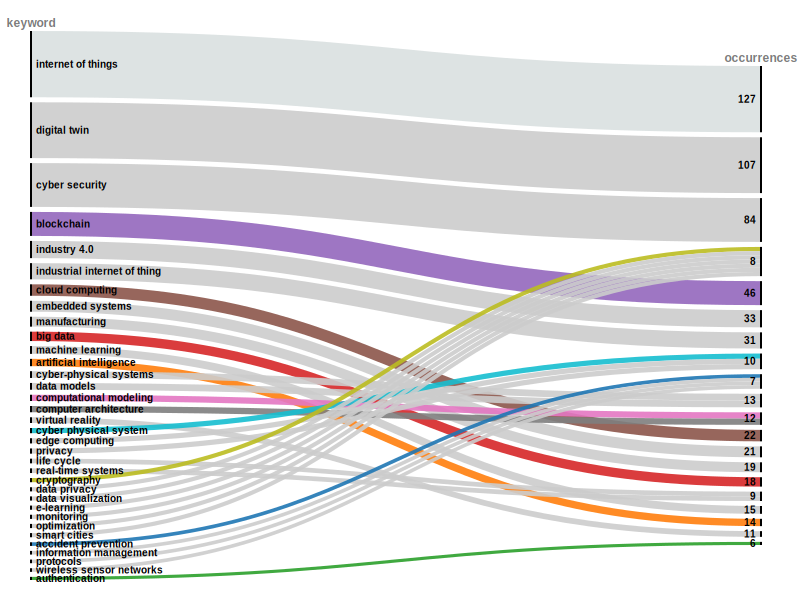
\includegraphics[width=\textwidth]{images/key_belt.png}
    \caption{Frequency of keywords}
    \label{fig:alluvial-key}
\end{figure}

Bibliographic information from 175 papers is used to generate 1187 keywords. Using thesaurus text file, we configure the tool to merge keywords that have similar semantic meaning. Moreover, we set a minimum threshold to limit the result to 87 keywords that meet 3 occurrences of the 1187 keywords.    


The analyisis of the selected papers using VOSviewer software revealed that which terms were frequently mentioned on the abstract and keyword section of the paper. The most frequently mentioned terms were "digital twin" with 72 occurrences, followed by "cybersecurity" with 66 occurrences, "cyberphysical system" with 24 occurrences, "cyber attacks" with 20 occurrences, "internet of things" with 19 occurrences, and "embedded systems" with 17 occurrences.This analysis highlights the key themes and concepts that are prevalent in current research on the topic of Digital Twin and IoT security. The high frequency of the term "digital twin" indicates the centrality of this concept in the field and the importance of understanding its role in ensuring the security of industries utilizing DT and IoT applications. The frequent mention of terms such as "cybersecurity" and "cyber attacks" further emphasizes the need for robust security measures to protect these systems from malicious actors.Additionally, the presence of terms such as "cyberphysical system" and "embedded systems" highlights the need for interdisciplinary research and collaboration between experts in fields such as computer science, engineering, and physics to effectively address the security challenges facing Digital Twin and IoT.

In order to gain further insights into the evolution of research in the field of Digital Twin and IoT security, a keyword co-relationship network analysis was extracted from VOSviewer tool. This analysis aimed to identify clusters of related items and to visualize the relationships between keywords over time. The results of this analysis revealed that in the early days of research on Digital Twin, keywords such as "monitoring", "safety", "prototypes", "resilience", "software", and "tools" were frequently mentioned, which suggests that the primary focus of research at that time was on utilizing Digital Twin as a visual aid. However, more recent research is characterized by the frequent mention of emerging technologies such as "blockchain," "machine learning," "e-learning" "5G," and "privacy" This indicates that the development of Digital Twin has shifted towards utilizing these technologies to enhance its security capabilities. This highlights the importance of continuous monitoring of the research field and to adapt to new technologies and approaches for Digital Twin security.



\begin{figure}[H]
    % \centering
    % \includegraphics[width=1.5\textwidth, center]{images/vos_key_cooc_6_final.png}
    \includesvg[width=\textwidth]{images/svg/vos_co_time_2.svg}
    % \includesvg[inkscapelatex=false,width=0.95\columnwidth]{images/key_belt.svg}
    \caption{keyword co-relationship from VOSviewer}
    \label{fig:co-occurrence-vosv}
\end{figure}

The analysis of the co-occurrence of keywords in the selected articles, as represented in Figure \ref{fig:co-occurrence-vosv}, reveals the identification of five clusters. These clusters, as defined by the VOSviewer documentation, are groups of terms that exhibit a high degree of relatedness. Cluster one encompasses terms related to 5G technology, machine learning, real-time security analysis, security frameworks, access control, and automation. Cluster two comprises of keywords such as cybersecurity, data models, digital twin, internet of things, privacy, prototypes, safety, and cloud computing. The third cluster encompasses terms such as those related to the automotive industry, availability, blockchain, industry 4.0, industrial control systems, system life cycle, intelligent control, software, and tools. The fourth cluster is comprised of analytical models, anomaly detection, cyber-attacks, monitoring, resilience, critical infrastructure, integrated circuits, and physical systems. The final cluster includes terms such as cyber-physical systems, e-learning, embedded systems, predictive models, and smart grids.
%----------------------------------------------------------------------------------------

% \subsection{Study Selection and Refinement}
%----------------------------------------------------------------------------------------
% ======================================================================================================
% NOTES, TODOS
% ======================================================================================================
\subsection{Study Selection and Refinement}
% 74 selected papers -> 14 not relevant and 3 duplicate studies submitted to different journals  excluded during full review of the papers. 

Even thought, we initially selected 73 papers for analysis. Upon further examination, we discovered three studies that were duplicates with different metadata but had similar content, and had been submitted to different journals. These duplicates were not identified by the tools we had used to exclude them. In addition, through quality assessment checklist, we also excluded fourteen papers for data extraction phase.

The reasons for the exclusion of these papers were as follows:

\begin{itemize}
    \item When the paper discussed how to secure the digital twin itself, rather than securing IoT applications using digital twin technology or securing the communication channel between DT and (I)IoT. 
    \item If the paper lacked a clear objective and aim.
    \item Some were not related to securing (I)IoT applications with an Industry 4.0 use case (for example, a study that used a digital twin to secure a data centre).
    \item Study sourced from book chapter. 
    \item The study was not relevant to any of the research questions.
    \item A study that focuses on securing (I)IoT devices that are not associated with any industry use case. 
\end{itemize}

As a result of this refinement and selection process, we were left with final set of 56 papers that were used for data extraction and analysis. In the following chapter, we provide a review of the 56 papers focusing to answer two research questions: How is digital twin used to improve the security of (I)IoT applications and what security mechanisms are used to secure the communication channel?    




%----------------------------------------------------------------------------------------

% \subsection{Data Extraction and Monitoring}
%----------------------------------------------------------------------------------------
% ======================================================================================================
% NOTES, TODOS
% ======================================================================================================
\subsection{Data Extraction and Monitoring}
%----------------------------------------------------------------------------------------

% \subsection{Data Synthesis}
%----------------------------------------------------------------------------------------
% ======================================================================================================
% NOTES, TODOS
% ======================================================================================================
\subsection{Data Synthesis}
%----------------------------------------------------------------------------------------







%----------------------------------------------------------------------------------------

% Todo: Method for data extraction and synthesis 
% \subsection{Data Extraction Method}
% \subsection{Data Synthesis Method} 
% Chapter 3
% ======================================================================================================
% NOTES, TODOS
% ======================================================================================================


\chapter{Preliminaries} 
\label{Chapter3}


This research has 3 main components worth to describe them here. These are lightweight encryption, IoT device, Digital Twin and MQTT protocol. In this section, we provide background of each element from its relevance to the project. 

\section{Lightweight Encryption/Authentication }


Authenticate encryption is a method of providing confidentiality and message integrity at the same time with one call of operation. While confidentiality comes from the generated cypher, authentication or integrity comes from the tag generated during encryption. Upon receiving, the receiver can decrypt the cypher to get the plan message as well as check the tag is the same in order to check neither the message nor the cypher has been modified upon transmission.

\subsection{AES-GCM}


\subsection{ASCON}

ASCON is an authenticate encryption algorithm designed and developed by A, B, C and at University. Though it has been under the curtain for years, it become very popular after it wins CASEAR NIST computation. The authors claim the main goal of the algorithm is to provide simplicity, online, security, side-channel robustness, single-pass and lightweight cipher for the resource-constrained device. It is is also a well-performing algorithm for short messages \cite{dobraunigAsconV1Lightweight2021} like for applications to collect environment and operating condition in industry 4.0

The algorithm can also be used on high-performin machines to provide encryption and decryption for  time-critical applications. It can provide 128-bit key security \cite{dobraunigAsconV1Lightweight2021}, surpassing the currently accepted 80-bit security standard.


\begin{figure}[H]
    \centering
    \caption{ASCON encryption }
    \includegraphics{images/fp/aead_encrypt.pdf}
    \label{fig:ascon-enc}
\end{figure}

The encryption and decryption process of ASCON is split into 4 main phases is depicted in Figure \ref{fig:ascon-enc, fig:ascon-dec}. These are initialization, associated data processing, plain text/cipher text processing (depending on whether it is in encryption or decryption mod) and finalization. 



\begin{figure}[H]
    \centering
    \caption{ASCON decryption}
    \includegraphics{images/fp/aead_decrypt.pdf}
    \label{fig:ascon-dec}
\end{figure}

\section{(Industry) Internet of Things }
\input{sections/fp/Chapter6/dt}
\input{sections/fp/Chapter6/mqtt}


\include{chapters/chapter4} 
\include{chapters/chapter5} 



%----------------------------------------------------------------------------------------
%	THESIS CONTENT - APPENDICES
%----------------------------------------------------------------------------------------

\appendix % Cue to tell LaTeX that the following "chapters" are Appendices

% Include the appendices of the thesis as separate files from the Appendices folder
% Uncomment the lines as you write the Appendices

% % Appendix Template

\chapter{AppendixA: Proof of Concept Application Source Code } % Main appendix title

\label{AppendixA} % Change X to a consecutive letter; for referencing this appendix elsewhere, use \ref{AppendixX}

This appendix provides the main source code for the proof of concept application development based on our proposed solution. Note that, the source code for each encryption cryptography algorithm used in this paper is taken from the respective official GitHub repository. 

In addition, various lines of code are indicated and commented on to show how we perform measurements for latency, memory usage and UART logging for power analysis. 


\begin{lstlisting}[style=CStyle, caption={Main Source C File of The Proposed Implementation}, label={list:mainc-ascon}]

#include <Arduino.h>
#include <WiFi.h>
#include <sstream>
#include <iomanip>
#include <PubSubClient.h> // MQTT Client
// #include <time.h>
#include <esp_timer.h>
#include <esp_system.h>
#include <xtensa/core-macros.h>
// for generating nonce
#include <iostream>
#include <random>
#include <chrono>
// Libaries for UART
#include "driver/uart.h"
#include "driver/gpio.h"


extern "C" {
  #include "api.h"
  #include "core.h"
}

const char*  ssid         = "Linawifi";
const char*  password     = "Wifi3364";

const char*  mqtt_server  = "65.21.107.159";
const int    mqtt_port    = 1883;
const char*  mqtt_user    = "";
const char*  mqtt_pass    = "";


/*----------------------------------------------------------------------*/
// Define UART number for communication with the GPS.
/*----------------------------------------------------------------------*/
static const int RX_BUF_SIZE = 1024;

// Define TX and RX pins for the GPS.
#define TXD_PIN (GPIO_NUM_17)
#define RXD_PIN (GPIO_NUM_16)

// Define UART as number 2
#define UART UART_NUM_2


int num = 0;

/*----------------------------------------------------------------------*/



/*----------------------------------------------------------------------*/
// Function to generate random nonce of size 'size'
/*----------------------------------------------------------------------*/
std::string generateNonce(int size) {
    std::random_device rd;
    std::mt19937 gen(rd());
    std::uniform_int_distribution<> dis(0, 255);

    std::string nonce;
    for (int i = 0; i < size; ++i) {
        nonce += static_cast<char>(dis(gen));
    }

    return nonce;
}
/*----------------------------------------------------------------------*/


WiFiClient   wifi_client;
PubSubClient pubsub_client(wifi_client);


int encrypt_payload_ascon(unsigned char *p_cipher, unsigned char *payload, unsigned char *thingid){
     // Specify the size of the nonce you want to generate (in bytes)
    int nonceSize = 16; // Both ASCON and AES-GCM typically uses a 12-byte nonce
    // Generate a nonce
    std::string generatedNonce = generateNonce(nonceSize);

    // Convert the generated nonce to a const char array
    // const char nonce[] = "0123456789abcdef";
    const char *nonce = generatedNonce.c_str();

    unsigned char n[CRYPTO_NPUBBYTES]; 
    memcpy(n, nonce, sizeof(n));

    const char key[] = "thisismysymekey1";
    unsigned char k[CRYPTO_KEYBYTES];
    memcpy(k, key, sizeof(k));

    unsigned char *a = thingid;
    unsigned char *m = payload;
    // unsigned char c[32];

    unsigned long long alen = 16;
    unsigned long long mlen = 16;
    unsigned long long clen = CRYPTO_ABYTES;


    int result = 0;
    /* ======================= Cycle Count ======================= */
    // get esp cycle count
    // uint32_t StartCycleCount = xthal_get_ccount(); 


    /* ======================= Execution time ======================= */
    // //  Start the timer
    // uint64_t startTime = esp_timer_get_time();

    /* ======================= Memory Usage ======================= */
    // measure memory usage before the function call
    // uint32_t free_memory_before = esp_get_free_heap_size();
    // printf("Free memory before: %d bytes\n", free_memory_before);
    // Print the total heap size

    /* ======================= Function call ======================= */
    const char* logmsg = "[encrypt_payload_ascon] calling crypto_aead_encrypt-ascon.\n";
    uart_write_bytes(UART, logmsg, strlen(logmsg));
    result |= crypto_aead_encrypt(p_cipher, &clen, m, mlen, a, alen, (const unsigned char*)0, n, k);
    const char* logmsg2 = "[encrypt_payload_ascon] calling crypto_aead_encrypt-ascon.\n";
    uart_write_bytes(UART, logmsg2, strlen(logmsg2));

  
    /* ======================= End Cycle Count ======================= */
    // get endcyclecount using esp cycle count
    // uint32_t endCycleCount = xthal_get_ccount();

    // uint32_t cycleCount = endCycleCount - StartCycleCount;
    // size_t total_bytes = 64;
    // double cb_ratio = (double)cycleCount / total_bytes;
    // double throughput = (double)1 / cb_ratio;
    // // // print cycle count
    // printf("Cycle count:cc %u cb_ratio: %f throughput: %f\n", cycleCount, cb_ratio, throughput);
    
    
    /* ======================= End Execution time ======================= */
    // // Stop the timer
    // uint64_t endTime = esp_timer_get_time();
    // // Calculate the execution time
    // uint64_t executionTime = endTime - startTime;
    // // print execution time
    // printf("Execution time-alg: %llu microseconds\n", executionTime);

    /* ======================= End Memory Usage  Measureent=================== */
    // uint32_t free_memory_after = esp_get_free_heap_size();
    // // calculate the memory used by the function call
    // uint32_t memory_used = free_memory_before - free_memory_after;
    // // print memory used
    // printf("Memory used: %d bytes\n", memory_used);

    return result;
 }

unsigned char* const_char_to_unsigned_char(const char* p_str){
    // Input
    const char* str = p_str;
    size_t len = strlen(str);

    // Process
    // The following block of code is not secure as we are not considering to write null character at the end 
    // of the string.
    unsigned char* result = (unsigned char*)malloc(len);
    if(result != NULL){
        memcpy(result, str, len);
        // result[len] = '\0';
    }

    // Ouput 
    return result;
}

std::string float_to_string(float value) {
  std::ostringstream stream;
  stream << std::fixed << std::setprecision(2) << value;
  return stream.str();
}

std::string convertToHexString(const unsigned char* ptr, size_t size) {
    std::string hexString;
    hexString.reserve(size * 2); // Reserve space for the hexadecimal representation

    for (size_t i = 0; i < size; i++) {
        char hexBuffer[3];
        snprintf(hexBuffer, sizeof(hexBuffer), "%02x", static_cast<unsigned int>(ptr[i]));
        hexString += hexBuffer;
    }

    return hexString;
}

void publish_temperature_data(float value, float p_altitude) {
    // Construct topic string.
    std::string username(mqtt_user, 7);
    // std::string topic = "temperature/" + username + "/sensor";
    std::string topic = "ut-sensors";

    // Convert temperature to a string message.
    std::string tempstr = float_to_string(value);
    std::string altistr = float_to_string(p_altitude);

    const char payloadcc[] = "{\"tem\":7,\"al\":3}";
    unsigned char payloaduc[16]; 
    memcpy(payloaduc, payloadcc, sizeof(payloaduc));

    const char thingIdcc[] = "ut-sensors:esp01";
    unsigned char thingIduc[16];
    // Copy the string literal to unsigned char type variable 
    memcpy(thingIduc, thingIdcc, sizeof(thingIduc));

    unsigned char cipher[32];

    int result = 0;
    const char* logmsg = "[publish_temperature_data] calling encryption function-ascon.\n";
    uart_write_bytes(UART, logmsg, strlen(logmsg));
    result |= encrypt_payload_ascon(cipher, payloaduc, thingIduc);
    const char* logmsg2 = "[publish_temperature_data] end of encryption function call-ascon.\n";
    uart_write_bytes(UART, logmsg2, strlen(logmsg2));
    

    // std::string payloadEncr = encrypt_payload_ascon(payloadText,  );
    // "{\"payload\":\"bb6e50f539fbd657efe8021a19d101178289d87ccbc056348fd0d08fbc150528\",\"tid\":\"ut-sensors:esp01\"}"
    //{"payload":"e23841fd76e3d95682097eaafb38f7796fac95ed47e18bbb1ffd5f8d223e7a49","tid":"ut-sensors:esp01"}
    std::string payload = "{\"payload\":\"";
    // std::string payload_val = std::string(reinterpret_cast<char*>(cipher), sizeof(cipher));
    std::string payload_val = convertToHexString(cipher, 32);
    std::string tid = "\",\"tid\":";
    std::string tid_val = "\"ut-sensors:esp01\"}";

    std::string msg2 = payload + payload_val + tid + tid_val;

    // Serial.print("Publishing temperature data [");
    // Serial.print(topic.c_str());
    // Serial.print("] ");
    // Serial.println(msg2.c_str());
    // a1bd73dfea710f93e2782e50284d4c17a7be0d9a62114937fe34b2a32c16fae7
    // Publish!
    pubsub_client.publish(topic.c_str(), msg2.c_str(), msg2.length());
    // #MEM
    // printf("[publish_temparature_data]:Freep Heap Size Level 2 : %d bytes  minimum: %d bytes\n", esp_get_free_heap_size(), esp_get_minimum_free_heap_size()); 
}

void setup() {
  // Connect the board to wife access.
    Serial.begin(115200);
    WiFi.begin(ssid, password);
    delay(10000);


    // Initialize the UART connected to the GPS.
    const uart_config_t uart_config = {
        .baud_rate = 115200,
        .data_bits = UART_DATA_8_BITS,
        .parity    = UART_PARITY_DISABLE,
        .stop_bits = UART_STOP_BITS_1,
        .flow_ctrl = UART_HW_FLOWCTRL_DISABLE,
        .source_clk = UART_SCLK_APB,
    };

    // Install UART driver
    uart_driver_install(UART, RX_BUF_SIZE * 2, 0, 0, NULL, 0);
    uart_param_config(UART, &uart_config);
    uart_set_pin(UART, TXD_PIN, RXD_PIN, UART_PIN_NO_CHANGE, UART_PIN_NO_CHANGE);


    const char* test_str = "[Setup] Entering to main function.\n";
    uart_write_bytes(UART, test_str, strlen(test_str));

    // #MEM
    Serial.print("[setup]Total Heap Size First--->>: ");
    Serial.print(ESP.getHeapSize());
    Serial.println(" bytes");


    // Keep trying to reconnect if not connected yet.
    while (WiFi.status() != WL_CONNECTED) {
        delay(500);
        Serial.println("Connecting to WiFi...");
    }

    // Set up the mqtt server configuration.
    pubsub_client.setServer(mqtt_server, mqtt_port);
}

void reconnect() {
    // Loop until we're reconnected
    while (!pubsub_client.connected()) {
        Serial.print("Attempting MQTT connection...");

        // Attempt to connect
        if (pubsub_client.connect("", mqtt_user, mqtt_pass)) {
            Serial.println("connected");
        } else {
            Serial.print("failed, rc=");
            Serial.print(pubsub_client.state());
            Serial.println(" try again in 5 seconds");
            delay(5000);
        }
    }
}

void loop() {
    static int loopCounter = 0; 

    loopCounter++;

    
    // Get sensor values.
    float temperature = 9;
    float altitude = 4;

    // Reconnect if we lost connection.
    if (!pubsub_client.connected()) {
        reconnect();
    }
    // #MEM
    // printf("[loop]:Freep Heap Size Level 1: %d bytes  minimum: %d bytes\n", esp_get_free_heap_size(), esp_get_minimum_free_heap_size()); 

    if(loopCounter < 1000) {
        /* ======================= Execution time ======================= */
        // Start the timer
        // uint64_t startTime = esp_timer_get_time();

        /* ======================= RAM Memory Usage ====================== */
        // printf("[loop]:Freep Heap Size Level free: %d bytes  minimum: %d bytes\n", esp_get_free_heap_size(), esp_get_minimum_free_heap_size()); 


        // publish the sensor values 
        // *****************************************************************
        // ******************Function Call *****************************
        //
        printf("[loop]: Calling publish_temperature_data function-ascon.\n");
        publish_temperature_data(temperature, altitude);

        // 
        // ******************Function End ******************************
        //******************************************************************


        /* ======================= End Execution time ======================= */
        // // Stop the timer
        // uint64_t endTime = esp_timer_get_time();
        //  // Calculate the execution time
        // uint64_t executionTime = endTime - startTime;
        // // print execution time
        // printf("Execution time-app: %llu microseconds\n", executionTime);
    }

    // Update internal loops in mqtt client.
    pubsub_client.loop();


    // Wait for 2s before we read and publish the next sensor value.
    // Uncomment this line of code during power measurement 
    if (loopCounter % 100 == 0){
        delay(10000);
    }
    delay(500);
}
\end{lstlisting}

%% Appendix Template

\chapter{AppendixB:  } % Main appendix title

\label{AppendixB} % Change X to a consecutive letter; for referencing this appendix elsewhere, use \ref{AppendixX}

This appendix provides a code snippet that filters search results based on the presence of the term "digital twin" in the title of each paper. Specifically, the script used to extract search results from Springer Link. 


\begin{lstlisting}[language=Python, style=CStyle, caption={A python code snippet to identify papers which have "digital twin" in their title }, label={list:mainc-ascon}]

import csv

import re

 
counter = 0

results_file = '../data/SpringerLink_130523.csv'

accepted_filename = "../data/SpringerLink_130523_accepted.csv"

accepted_rows = []

 

with open(results_file, newline='', encoding="utf-8", errors="ignore") as fromfile:

    freader = csv.DictReader(fromfile, delimiter=';')

 

    for row in freader:

        counter += 1

        found = re.search(r'digital[\s-]{1}twin[s]?', row['Item Title'].lower())

 

        if found:

            accepted_rows.append(row)

 

with open(accepted_filename, 'w', newline='') as tofile:

    writer = csv.DictWriter(tofile, fieldnames=freader.fieldnames, delimiter=";")

    writer.writeheader()

    writer.writerows(accepted_rows)

 

print("count of papers:", counter)

print("count of papers with 'digital twin' in title:", len(accepted_rows))
\end{lstlisting}

%\include{Appendices/AppendixC}

%----------------------------------------------------------------------------------------
%	BIBLIOGRAPHY
%----------------------------------------------------------------------------------------

% \printbibliography[heading=bibintoc]
\printbibliography
%\bibliography{sources}

%----------------------------------------------------------------------------------------
\end{document}